% -*- coding: utf-8 -*-
\documentclass[serif]{beamer} %
%\usepackage[UTF8]{ctex}
%\usepackage{graphicx}
\usepackage[T1]{fontenc} % Needed for Type1 Concrete
\usepackage{concmath} % Concrete + Concmath

\setbeamertemplate{bibliography item}[text]

%\usetheme{Frankfurt}
\setbeamercolor{math text}{fg=blue}
\setbeamercovered{transparent}

\usepackage{pgf,tikz} % drawing
\usetikzlibrary{calc}
\usetikzlibrary{snakes,arrows,shapes}
\usepackage{amsmath}
\usepackage{amsthm}

\usepackage{xcolor}
\definecolor{mygreen}{rgb}{0,0.6,0}
\definecolor{mygray}{rgb}{0.5,0.5,0.5}
\definecolor{mymauve}{rgb}{0.58,0,0.82}
\definecolor{myblue}{rgb}{0.0,0.0,0.6}

\usepackage{listings}
\lstset{
  language=Matlab,
  basicstyle=\scriptsize\ttfamily\color{myblue},
  keywordstyle=\bfseries\color{blue},
  stringstyle=\color{mymauve},
  commentstyle=\itshape\color{mygreen},
  identifierstyle=\color{black},
  frame=L,
  numbers=left,
  numberstyle=\tiny\color{mygray}
}

%\usetheme{Madrid}
%\setbeamercovered{transparent}
\title[n_sphere]
{Sampling with Halton Points on n-Sphere}
%\subtitle{(confidential)}
%\author[陆伟成] % short version of author list (optional)
\author[Luk]
{Wai-Shing~Luk\inst{1}} % author list
%\institute[復旦] % short version of institution name (optional)
\institute[Fudan]
{ % institution name
  \inst{1}%
  School of Microelectronics\\
  Fudan University
}
\date[\today] % short version of date informations (optional)
{\today} % date informations
%\subject{Informatics} % visible in PDF properties data (optional)

\AtBeginSection[]
{
  \begin{frame}
    \frametitle{Agenda}
    \tableofcontents[currentsection]
  \end{frame}
}

\begin{document}
\definecolor{zzttqq}{rgb}{0.6,0.2,0}
\definecolor{qqqqff}{rgb}{0,0,1}

\begin{frame}[fragile]
  \titlepage
\end{frame}

\begin{frame}
  \frametitle{Agenda}
  \tableofcontents
\end{frame}

\section{Abstract}
%----------------------------------------------------
\begin{frame}[fragile]
\frametitle{Abstract}
\begin{itemize}
  \item Sampling on $n$-sphere ($S^n$) has a wide range of applications, such as:
      \begin{itemize}
        \item Spherical coding in MIMO wireless communication
        \item Multivariate empirical mode decomposition
        \item Filter bank design
      \end{itemize}
  \item We propose a simple yet effective method which:
      \begin{itemize}
        \item Utilizes low-discrepancy sequence
        \item Contains only 10 lines of MATLAB code in our implementation!
        \item Allow incremental generation.
      \end{itemize}
  \item Numerical results show that the proposed method outperforms the randomly generated sequences and other proposed methods.
\end{itemize}
\end{frame}

\section{Motivation and Applications}

\begin{frame}[fragile]
\frametitle{Problem Formulation}
Desirable properties of samples over $S^n$
\begin{itemize}
  \item Uniform
  \item Deterministic
  \item Incremental
  \begin{itemize}
    \item The uniformity measures are optimized with every new point.
    \item Reason: in some applications, it is unknown how many points are needed to solve the problem in advance
  \end{itemize}
\end{itemize}
\end{frame}

%\subsection{Motivation}

\begin{frame}[fragile]
\frametitle{Motivation}
\begin{itemize}
  \item The topic has been well studied for sphere in 3D, i.e. $n=2$
  \item Yet it is still unknown how to generate for $n > 2$.
  \item Potential applications (for $n > 2$):
  \begin{itemize}
    \item Robotic Motion Planning ($S^3$ and SO(3))~\cite{yershova2010generating}
    \item Spherical coding in MIMO wireless communication~\cite{utkovski2006construction}:
    \begin{itemize}
      \item Cookbook for Unitary matrices
      \item A code word = a point in $S^n$
    \end{itemize}
    \item Multivariate empirical mode decomposition~\cite{rehman2010multivariate}
    \item Filter bank design~\cite{mandic2011filter}
  \end{itemize}
\end{itemize}
\end{frame}


%----------------------------------------------------
\begin{frame}[fragile]
\frametitle{Halton Sequence on $S^n$}
\begin{itemize}
  \item Halton sequence on $S^2$ has been well studied~\cite{cui1997equidistribution} by using cylindrical coordinates.
  \item Yet it is still little known for $S^n$ where $n>2$.
  \item
\begin{alert}{Note:}
The generalization of cylindrical coordinates does NOT work in higher dimensions.    
\end{alert}

\end{itemize}
\end{frame}



\section{Review of Low Discrepancy Sequence}

\subsection{Van der Corput sequence on $[0,1]$}

\begin{frame}[fragile]
\frametitle{Basic: Van der Corput sequence}
\begin{itemize}
  \item Generate a low discrepancy sequence over $[0,1]$
  \item Denote $\mathrm{vd}(k,b)$ as a Van der Corput sequence of $k$ points, where $b$ is the base of a prime number.
  \item MATLAB source code is available at
  \url{http://www.mathworks.com/matlabcentral/fileexchange/15354-generate-a-van-der-corput-sequence }
\end{itemize}
\begin{example}
% \centerline{
%    \begin{tikzpicture}[>=latex',line join=bevel]
%        %\draw[help lines] (0,0) grid +(10,3);
%        \draw (0,1) -- (10,1); \pause
%        \draw (5,1) circle (2pt); \pause
%        \draw (2.5,1) circle (2pt); \pause
%        \draw (7.5,1) circle (2pt); \pause
%        \draw (1.25,1) circle (2pt); \pause
%        \draw (6.25,1) circle (2pt); \pause
%        \draw (3.75,1) circle (2pt); \pause
%        \draw (8.75,1) circle (2pt); \pause
%        \draw (0.625,1) circle (2pt); \pause
%        \draw (5.625,1) circle (2pt); \pause
%        \draw (3.125,1) circle (2pt); \pause
%        \draw (8.125,1) circle (2pt); \pause
%        \draw (1.875,1) circle (2pt); \pause
%        \draw (6.875,1) circle (2pt); \pause
%        \draw (4.375,1) circle (2pt); \pause
%        \draw (9.375,1) circle (2pt); 
%    \end{tikzpicture}
%  }
  \end{example}
\end{frame}


\subsection{Halton sequence on $[0,1]$}
\begin{frame}[fragile]
\frametitle{Unit Square $[0,1] \times [0,1]$}
\begin{columns}
\begin{column}{0.45\textwidth}
Halton sequence: using 2 Van der Corput sequences with different bases.
\begin{example}
    $[x,y] = [\mathrm{vd}(k,2), \mathrm{vd}(k,3)]$
\end{example}
\end{column}
\begin{column}{0.45\textwidth}
%\centerline{
%\begin{tikzpicture}[line cap=round,line join=round,>=triangle 45,x=5cm,y=5cm]
%    %\begin{tikzpicture}[>=latex',line join=bevel]
%    %\clip(-4.3,-2.96) rectangle (11,11);
%    \draw (0,0) -- (1,0); 
%    \draw (1,0) -- (1,1);
%    \draw (1,1) -- (0,1); 
%    \draw (0,1) -- (0,0); \pause
%    %\draw (     0,      0) circle (2pt); \pause
%    \draw (0.5000, 0.3333) circle (2pt); \pause
%    \draw (0.2500, 0.6667) circle (2pt); \pause
%    \draw (0.7500, 0.1111) circle (2pt); \pause
%    \draw (0.1250, 0.4444) circle (2pt); \pause
%    \draw (0.6250, 0.7778) circle (2pt); \pause
%    \draw (0.3750, 0.2222) circle (2pt); \pause
%    \draw (0.8750, 0.5556) circle (2pt); \pause
%    \draw (0.0625, 0.8889) circle (2pt); \pause
%    \draw (0.5625, 0.0370) circle (2pt); \pause
%    \draw (0.3125, 0.3704) circle (2pt); \pause
%    \draw (0.8125, 0.7037) circle (2pt); \pause
%    \draw (0.1875, 0.1481) circle (2pt); \pause
%    \draw (0.6875, 0.4815) circle (2pt); \pause
%    \draw (0.4375, 0.8148) circle (2pt); \pause
%    \draw (0.9375, 0.2593) circle (2pt); \pause
%    \draw (0.0313, 0.5926) circle (2pt); \pause
%    \draw (0.5313, 0.9259) circle (2pt); \pause
%    \draw (0.2813, 0.0741) circle (2pt); \pause
%    \draw (0.7813, 0.4074) circle (2pt); \pause
%    \draw (0.1563, 0.7407) circle (2pt); \pause
%    \draw (0.6563, 0.1852) circle (2pt); \pause
%    \draw (0.4063, 0.5185) circle (2pt); \pause
%    \draw (0.9063, 0.8519) circle (2pt); \pause
%    \draw (0.0938, 0.2963) circle (2pt); 
%    \end{tikzpicture}
%  }
%\centerline{\includegraphics[width=0.9\textwidth]{Halton_sequence_2D}}
\end{column}
\end{columns}
\end{frame}

\subsection{Halton sequence on $[0,1]^n$}
\begin{frame}[fragile]
\frametitle{Unit Hypercube $[0,1]^n$}
\begin{itemize}
  \item Generally we can generate Halton sequence in a unit hypercube $[0,1]^n$:
  \[
  [x_1, x_2, \ldots, x_n] = [\mathrm{vd}(k,b_1), \mathrm{vd}(k,b_2), \ldots, \mathrm{vd}(k,b_n)]
  \]
  \item A wide range of applications on Quasi-Monte Carlo Methods (QMC).
\end{itemize}
\end{frame}

\subsection{Unit Circle $S^1$}
\begin{frame}[fragile]
\frametitle{Unit Circle $S^1$}
\begin{columns}
\begin{column}{0.6\textwidth}
  Can be generated by mapping the Van der Corput sequence to $ [0, 2\pi]$
  \begin{itemize}
    \item $\theta = 2\pi \cdot \mathrm{vd}(k,b)$
    \item $[x, y] = [\cos\theta, \sin\theta]$
  \end{itemize}
\end{column}
\begin{column}{0.4\textwidth}
%\centerline{
%\begin{tikzpicture}[line cap=round,line join=round,>=triangle 45,x=2cm,y=2cm]
%   \draw (0,0) circle (1); \pause
%   \draw ( 1.0000,       0) circle (2pt); \pause
%   \draw (-1.0000,  0.0000) circle (2pt); \pause
%   \draw ( 0.0000,  1.0000) circle (2pt); \pause
%   \draw (-0.0000, -1.0000) circle (2pt); \pause
%   \draw ( 0.7071,  0.7071) circle (2pt); \pause
%   \draw (-0.7071, -0.7071) circle (2pt); \pause
%   \draw (-0.7071,  0.7071) circle (2pt); \pause
%   \draw ( 0.7071, -0.7071) circle (2pt); \pause
%   \draw ( 0.9239,  0.3827) circle (2pt); \pause
%   \draw (-0.9239, -0.3827) circle (2pt); \pause
%   \draw (-0.3827,  0.9239) circle (2pt); \pause
%   \draw ( 0.3827, -0.9239) circle (2pt); \pause
%   \draw ( 0.3827,  0.9239) circle (2pt); \pause
%   \draw (-0.3827, -0.9239) circle (2pt); \pause
%   \draw (-0.9239,  0.3827) circle (2pt); \pause
%   \draw ( 0.9239, -0.3827) circle (2pt);
%    \end{tikzpicture}
%  }
%\centerline{\includegraphics[width=0.9\textwidth]{Halton_sequence_2D}}
\end{column}
\end{columns}
\end{frame}

\subsection{Unit Sphere $S^2$}
\begin{frame}[fragile]
\frametitle{Unit Sphere $S^2$}
\begin{columns}
\begin{column}{0.6\textwidth}
  Has been applied for computer graphic applications~\cite{wong1997sampling}
  \begin{itemize}
    \item $[z, x, y]$ \\
      = $[\cos\theta, \sin\theta\cos\varphi, \sin\theta\sin\varphi]$ \\
      = $[z, \sqrt{1-z^2}\cos\varphi, \sqrt{1-z^2}\sin\varphi]$
    \item $\varphi = 2\pi\cdot\mathrm{vd}(k,b_1)$ \% map to $[0,2\pi] $
    \item $z = 2\cdot\mathrm{vd}(k,b_2) - 1$ \% map to $[-1,1]$
  \end{itemize}
\end{column}
\begin{column}{0.4\textwidth}
  \centerline{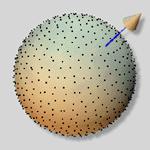
\includegraphics[width=0.8\textwidth]{thammer.png}}
\end{column}
\end{columns}
\end{frame}

\subsection{Sphere $S^n$ and SO(3)} % (fold)
\label{sub:sphere_s_n_and_so_3_}
\begin{frame}
  \frametitle{Sphere $S^3$ and SO(3)}
\begin{itemize}
  \item Deterministic point sets 
  \begin{itemize}
    \item Optimal grid point sets for $S^3$, SO(3) [Lubotzky, Phillips, Sarnak 86] [Mitchell 07]
  \end{itemize}
  \item No Halton sequences so far to the best of our knowledge
\end{itemize}
\end{frame}
% subsection sphere_s_n_and_so_3_ (end)

\section{Our approach}
\begin{frame}
  \frametitle{SO(3) or $S^3$ Hopf Coordinates}
\begin{columns}
\begin{column}{0.6\textwidth}
  \begin{itemize}
    \item Hopf coordinates (cf.~\cite{yershova2010generating})
    \begin{itemize}
      \item $x_1 = \cos(\theta/2) \cos(\psi/2)$
      \item $x_2 = \cos(\theta/2) \sin(\psi/2)$
      \item $x_3 = \sin(\theta/2) \cos(\varphi + \psi/2)$
      \item $x_4 = \sin(\theta/2) \sin(\varphi + \psi/2)$
    \end{itemize}
    \item $S^3$ is a principal circle bundle over the $S^2$
  \end{itemize}
\end{column}
\begin{column}{0.4\textwidth}
  \centerline{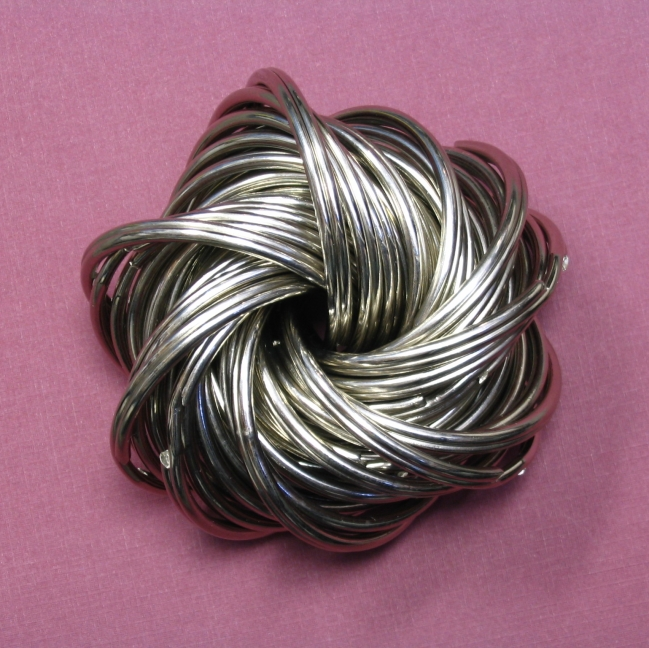
\includegraphics[width=0.8\textwidth]{Hopfkeyrings.jpg}}
\end{column}
\end{columns}
\end{frame}

\begin{frame}[fragile]
\frametitle{Hopf Coordinates for SO(3) or $S^3$}
  Similar to the Halton sequence generation on $S^2$, we perform the mapping:
  \begin{itemize}
    \item $\varphi = 2\pi\cdot\mathrm{vd}(k,b_1)$ \% map to $[0,2\pi] $
    \item $\psi = 2\pi\cdot\mathrm{vd}(k,b_2)$ \% map to $[0,2\pi] $ for SO(3), or
    \item $\psi = 4\pi\cdot\mathrm{vd}(k,b_2)$ \% map to $[0,4\pi] $ for $S^3$
    \item $z = 2\cdot\mathrm{vd}(k,b_3) - 1$ \% map to $[-1,1]$
    \item $\theta = \cos^{-1}z$
  \end{itemize}
\end{frame}

\begin{frame}[fragile]
\frametitle{10 Lines of MATLAB Code}
\begin{lstlisting}
function[s] = sphere3_hopf(k,b)
% sphere3_hopf   Halton sequence
varphi = 2*pi*vdcorput(k,b(1));   % map to [0, 2*pi]
psi = 4*pi*vdcorput(k,b(2));      % map to [0, 4*pi]
z = 2*vdcorput(k,b(3)) - 1;       % map to [-1, 1]
theta = acos(z);
cos_eta = cos(theta/2);
sin_eta = sin(theta/2);
s = [cos_eta .* cos(psi/2), ...
     cos_eta .* sin(psi/2), ...
     sin_eta .* cos(varphi + psi/2), ...
     sin_eta .* sin(varphi + psi/2)];
\end{lstlisting}
\end{frame}

\begin{frame}
  \frametitle{3-sphere}
  \begin{itemize}
    \item Polar coordinates:
    \begin{itemize}
      \item $x_0 = \cos\theta_3$
      \item $x_1 = \sin\theta_3 \cos\theta_2$
      \item $x_2 = \sin\theta_3 \sin\theta_2 \cos\theta_1$
      \item $x_3 = \sin\theta_3 \sin\theta_2 \sin\theta_1$
    \end{itemize}
  \end{itemize}
\end{frame}

\begin{frame}
  \frametitle{n-sphere}
  \begin{itemize}
    \item Polar coordinates:
    \begin{itemize}
      \item $x_0 = \cos\theta_n$
      \item $x_1 = \sin\theta_n \cos\theta_{n-1}$
      \item $x_2 = \sin\theta_n \sin\theta_{n-1} \cos\theta_{n-2} $
      \item $x_3 = \sin\theta_n \sin\theta_{n-1} \sin\theta_{n-2} \cos\theta_{n-3} $
      \item $\cdots$
      \item $x_{n-1} = \sin\theta_n \sin\theta_{n-1} \sin\theta_{n-2} \cdots \cos\theta_1$
      \item $x_n = \sin\theta_n \sin\theta_{n-1} \sin\theta_{n-2} \cdots \sin\theta_1$
    \end{itemize}
  \end{itemize}
\end{frame}

\begin{frame}
  \frametitle{How to Generate the Point Set}
  \begin{itemize}
    \item $p_0 = [\cos\theta_1, \sin\theta_1]$ where $\theta_1 = 2\pi\cdot\mathrm{vd}(k,b_1)$
    \item Let $f_j(\theta)$ = $\int\sin^j\theta \mathrm{d}\theta$, where $\theta\in (0,\pi)$. \\
    Note: $f_j(\theta)$ is a monotonic increasing function in $(0,\pi) $
    \item Map $\mathrm{vd}(k,b_j)$ uniformly to $f_j(\theta)$:\\
     $t_j = f_j(0) + (f_j(\pi) - f_j(0)) \mathrm{vd}(k,b_j)$
    \item Let $\theta_j = f_j^{-1}(t_j)$
    \item Define $p_n$ recursively as: \\
          $p_n = [\cos\theta_n, \sin\theta_n \cdot p_{n-1}]$
  \end{itemize}
\end{frame}

\begin{frame}
  \frametitle{$S^3$ projected on four different spheres}
  \centerline{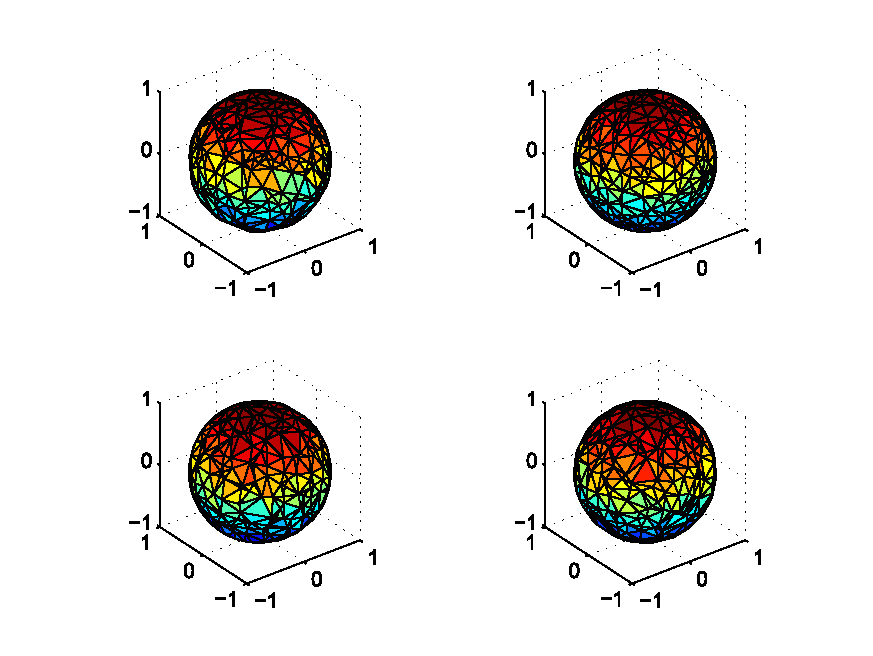
\includegraphics[width=0.9\textwidth]{res_proj.pdf}}
\end{frame}

%----------------------------------------------------
%% \begin{frame}[fragile]
%% \frametitle{MATLAB}
%% \begin{lstlisting}
%% function[p] = sphere_n(k,n,b)
%% % n_sphere
%% % INPUTS   :
%% %   k - maximum sequence index, non-negative integer
%% %   b - sequence base, integer exceeding 1
%% x0 = (2*pi)*vdcorput(k,b(1));  % map to [0, 2*pi]
%% p = [cos(x0), sin(x0)];
%% m = 3*k; % number of interpolation points
%% x = [0:pi/(m-1):pi];
%% for i=1:n-1
%%    syms a;
%%    t = subs(int(sin(a)^i), x);
%%    % map to [t1, tm]
%%    ti = t(1) + (t(m) - t(1)) * vdcorput(k,b(i+1));
%%    xi = interp1(t,x,ti,'spline');
%%    p = [cos(xi), sin(xi)*ones(1,i+1) .* p];
%% end
%% \end{lstlisting}
%% \end{frame}


\section{Numerical Experiments}

\begin{frame}
  \frametitle{Testing the Correctness}
  \begin{itemize}
    \item Compare the dispersion with the random point-set
    \begin{itemize}
      \item Construct the convex hull for each point-set
      \item Dispersion roughly measured by the difference of the maximum distance and the minimum distance between every two neighbour points: 
\[
      \max_{a \in \mathcal{N}(b)} \{D(a,b)\} - 
        \min_{a \in \mathcal{N}(b)} \{ D(a, b) \}  
\]
      where $D(a,b) = \sqrt{1 - a^\mathrm{T} b}$
    \end{itemize}
  \end{itemize}
\end{frame}

\begin{frame}
  \frametitle{Random sequences}
  \begin{itemize}
    \item To generate random points on $S^n$, spherical symmetry of the multidimensional Gaussian density function can be exploited.
    \item Then the normalized vector ($x_i/\|x_i\|$) is uniformly distributed over the hypersphere $S^n$. [Fishman, G. F. (1996)]
  \end{itemize}
\end{frame}


\begin{frame}
  \frametitle{Convex Hull with $\approx$400 points}
  \centerline{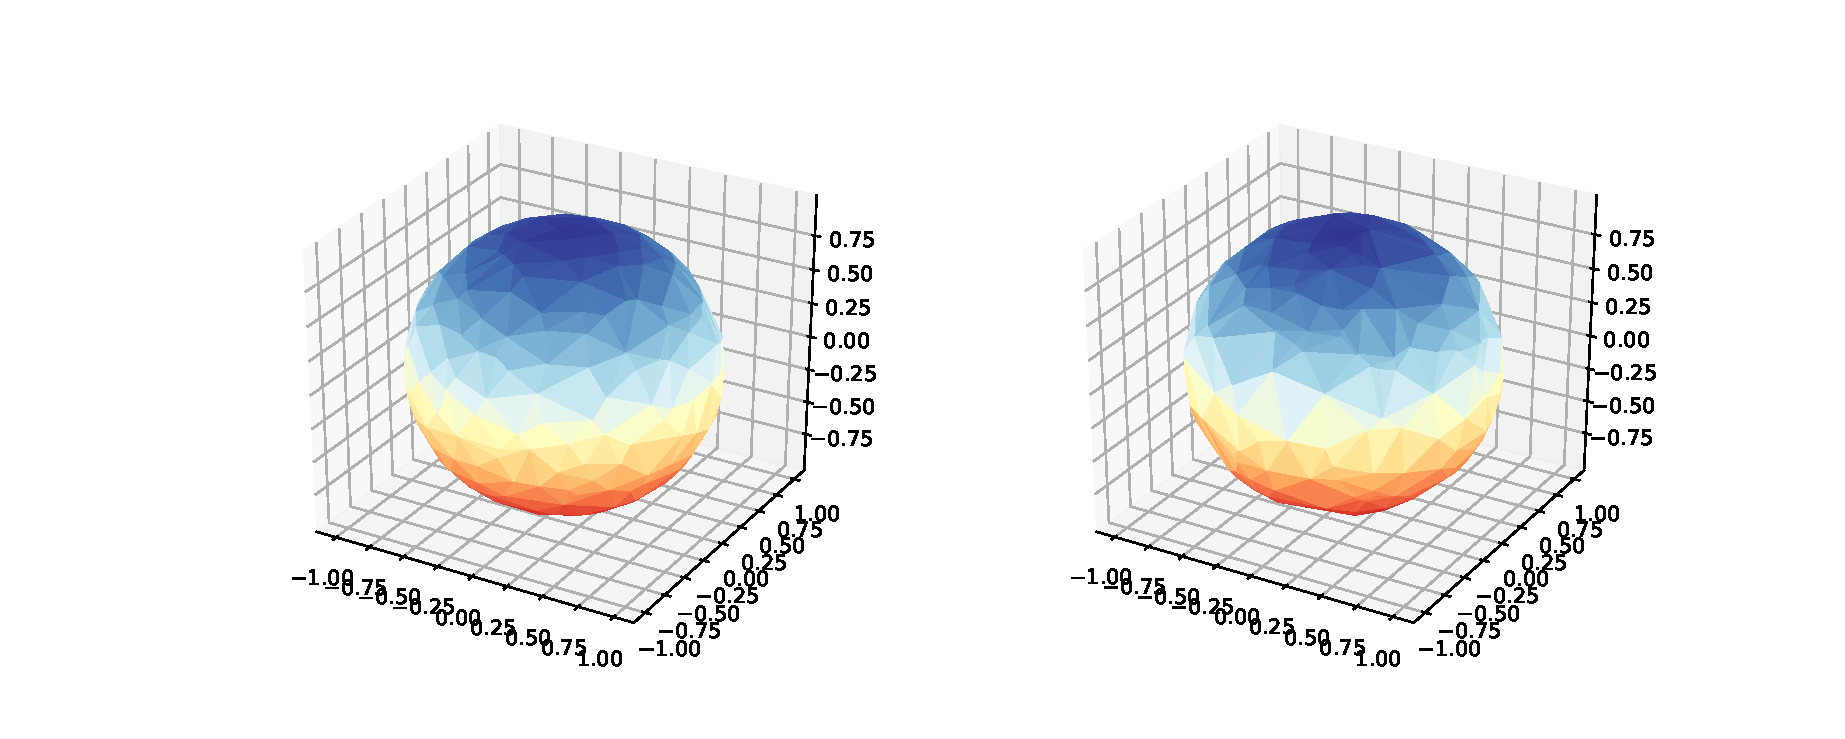
\includegraphics[width=0.9\textwidth]{res_compare.pdf}}
  Left: our, right: random
\end{frame}


\begin{frame}
  \frametitle{Result for $S^3$}
  \centerline{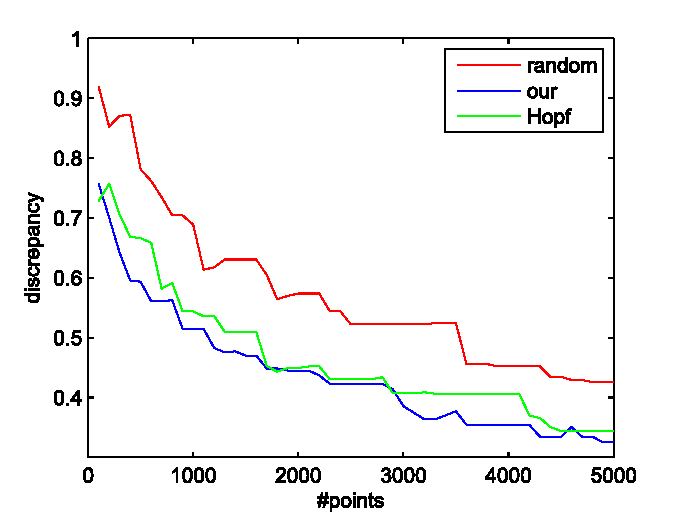
\includegraphics[width=0.9\textwidth]{res_hopf.pdf}}
\end{frame}

\begin{frame}
  \frametitle{Result for $S^4$}
  \centerline{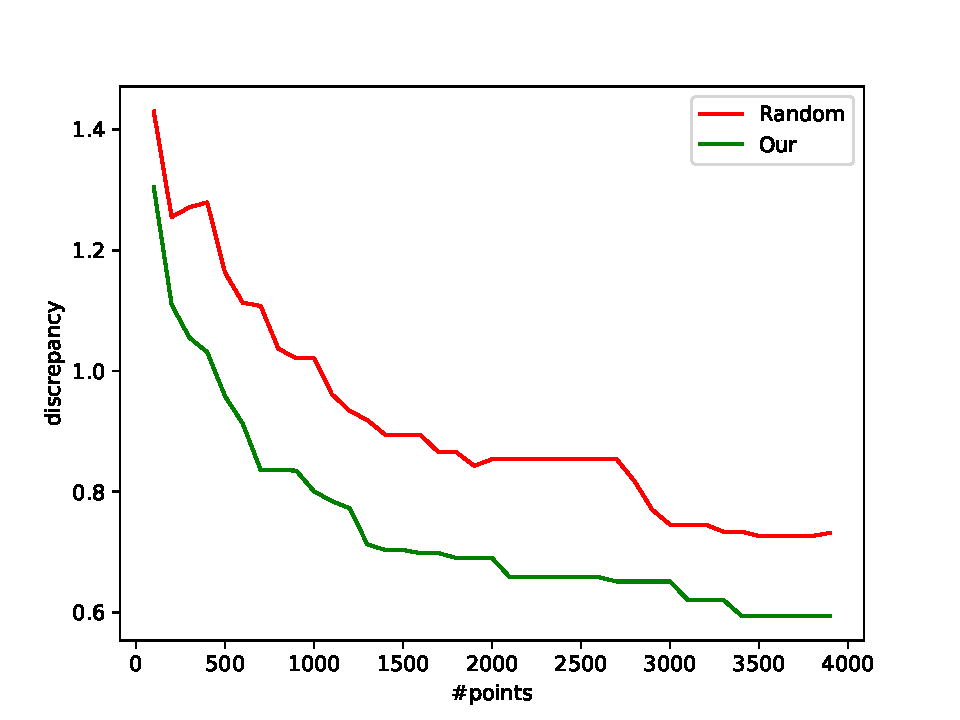
\includegraphics[width=0.9\textwidth]{res_S4.pdf}}
\end{frame}

\section{Conclusions}
\begin{frame}
  \frametitle{Conclusions}
  \begin{itemize}
    \item Proposed method generates low-discrepancy point-set in nearly linear time
    \item The result outperforms the corresponding random point-set, especially when the number of points is small
    \item The MATLAB source code is available in public (or upon request)
  \end{itemize}
\end{frame}

\begin{frame}[allowframebreaks]
  \frametitle{References}
  \scriptsize{\bibliographystyle{amsalpha}}
  %\bibliographystyle{amsalpha}
  \bibliography{n-sphere}
\end{frame}

\end{document}
